\chapter{Testing}

Detailed descriptions of every test case are definitely not what is required here. What is important is to show that you adopted a sensible strategy that was, in principle, capable of testing the system adequately even if you did not have the time to test the system fully.

Provide information in the body of your report and the appendix to explain the testing that has been performed. How does this testing address the requirements and design for the project?

How comprehensive is the testing within the constraints of the project?  Are you testing the normal working behaviour? Are you testing the exceptional behaviour, e.g. error conditions? Are you testing security issues if they are relevant for your project? 

Have you tested your system on ``real users''? For example, if your system is supposed to solve a problem for a business, then it would be appropriate to present your approach to involve the users in the testing process and to record the results that you obtained. Depending on the level of detail, it is likely that you would put any detailed results in an appendix.

The following sections indicate some areas you might include. Other sections may be more appropriate to your project. 

\section{Overall Approach to Testing}
The project used TDD as part of the process for software implementation. As well as designing features, tests were also designed for the required functions before functional code was written. There were two main types of tests for the website: unit tests that test the functionality of the model and the controllers and system tests that use selenium to check the flow of the system and simulate the actions of a user. Where appropriate, tests for functions were written to test three different cases:
\begin{itemize}
\item Success case: This would simulate either an expected input parameter for the function or an expected state that the system should be in in order to run it. 
\item Edge case: This would check the maximum functioning range of the function. For example if the function was only designed to allow 5 viewers to participate in a game, then it would check that the when the viewers total 5 the function still passes.
\item Failure case: This would ensure that given incorrect parameters or system state then the function would fail in the expected way.
\end{itemize}

For unit tests, tests were organised into classes were each test class would test a class or module of code. Similarly, system tests were designed to test a single Django template. The requirement for adding code to the master branch is that all unit and system tests (past and present) must pass and the static analysis tools must produce no errors.

\section{Automated Testing}
\subsection{Jenkins}
To improve the consistency of the code base, the GitHub repository was linked to a local Jenkins server. This server was set up at the beginning of the project and was used as part of the development life cycle of each feature. The Jenkins server ran as a background process on the development machine. The set up for the Jenkins server followed two guides: The official Jenkins Windows Service installation guide \textit{"Installing Jenkins as a Windows Service"} \cite{jenkins_wiki_install} from the Jenkins.io wiki and Steve's Blog \textit{"Automated python unit testing, code coverage and code quality analysis with Jenkins"} \cite{steves_blog} a self hosted technical blog from a software developing consultant specialising in Python.

Whilst Jenkins offers the ability to run tests periodically, this feature was not used and tests were triggered manually by the developer. The reasoning behind this is that incremental time based builds were not required. Had the project been developed by a team, the need for timed builds is more justifiable as many developers will be pushing code changes simultaneously. In a single person developer team, code is pushed one feature at a time and the work flow is linear hence there is no justifiable requirement for periodical builds. Despite this, the use of Jenkins is still admissible in a single developer project as it allows for centralised building of the project in a controlled, repeatable, environment. Additionally, The formatting for results produced by Jenkins offers an easy way to quickly visualise problems with the code base.

\subsection{Static analysis}
\subsubsection{Pylint}
Pylint is a linting tool that follows the PEP8 standards \cite{pep8} for python coding. The linter runs static analysis on the code base and ensures that all code meets with the standards specified by PEP8 (and produces warning and errors were this is not the case. The PEP8 standards include guidelines style and syntax as well as documentation (in the form of doc strings). Whilst several standards for the Python coding language are available, PEP8 was chosen as it is promoted by the developers of the Python language and is the most popular. An example of the Pylint output rendered by Jenkins is displayed below in Figure \ref{fig:jenkins_pylint}.
\begin{figure}[h!]
	\centering{
		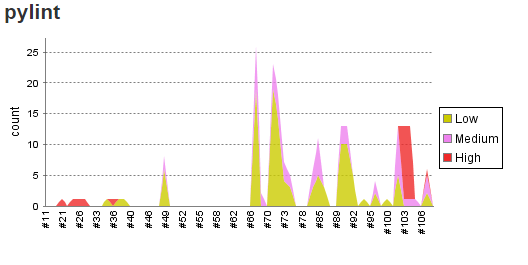
\includegraphics[scale=0.75]{Chapter4/jenkins_pylint.PNG}
		\caption{The output of the Pylint test run on the full code base rendered by Jenkins. Here, the number of warnings, and there severity, is logged by each build number. The peaks correspond to the first time a feature is pushed, these problems are then normally resolved in the troughs. In order to be able to merge a feature, the Pylint graph must be at zero warnings.}
		\label{fig:jenkins_pylint}
	}
\end{figure}

\subsubsection{Test coverage} 
An additional testing package, nosetest \cite{nosetest}, was used to run python tests for this project. This package, amongst other advantages, produces reports that are interpretable by Jenkins for both unit tests and test coverage. As the web based charades game was written in Django (which has its own testing framework), noetest could only be used for the hologram creation software. The test coverage displays graphically the proportion of the code that is run in tests. Although basic, this helps to highlight potential conditional statements, function and even lines that are not being tested. An example of the test coverage output rendered by Jenkins is displayed below in Figure \ref{fig:jenkins_test_cover}. Figure \ref{fig:jenkins_test_cover} shows that whilst the majority of the code base is covered by testing, several lines in the python.vpa package are excludes. These lines had to be omitted from tests as their functionality was to the perform the video processing loop. Whilst the functions that are called within that loop are sufficiently tested, the loop itself can not be tested easily as it creates an output window. The output window is only successfully closed via mouse click on the window close button (an operation not easily replicated in tests).
\begin{figure}[h!]
	\centering{
		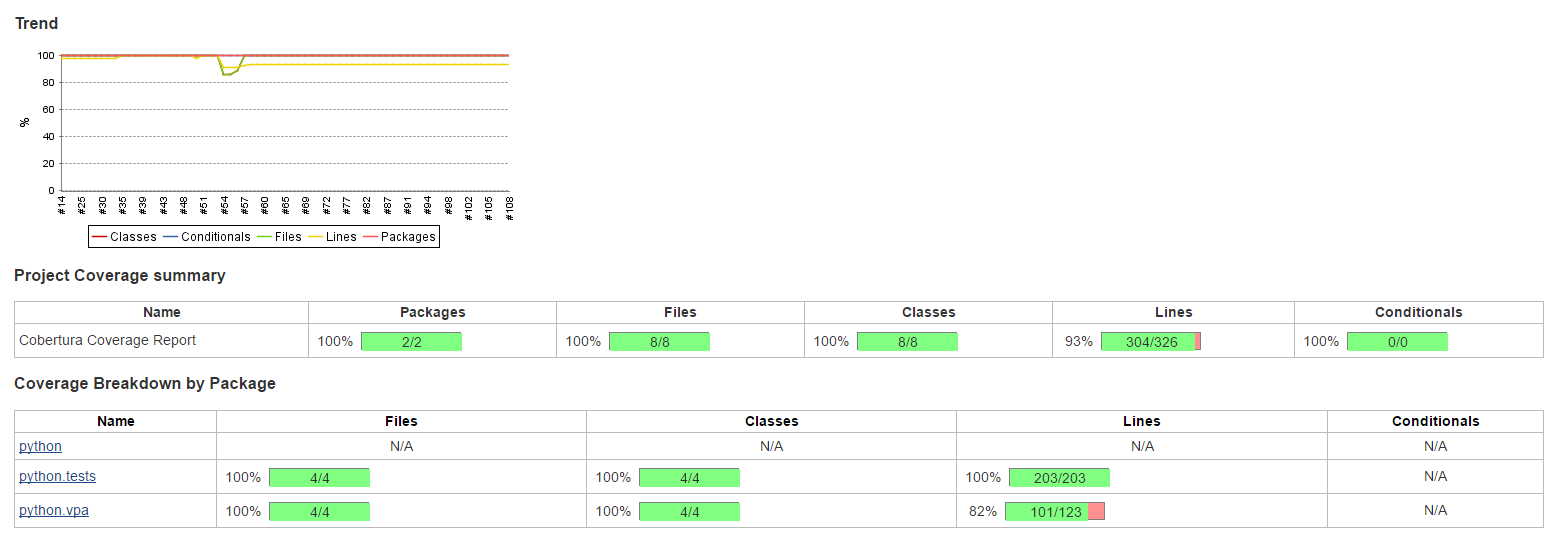
\includegraphics[scale=0.75]{Chapter4/jenkins_test_coverage.PNG}
		\caption{The above shows the rendered output of the test coverage report from nosetest in Jenkins. This report includes both a graphical and table representation of the data showing the amount of code that is being exercised by the unit tests. Note the incomplete test coverage and see explanation above.}
		\label{fig:jenkins_test_cover}
	}
\end{figure}
 

\subsection{Unit Tests}


\subsection{User Interface Testing}

\subsection{Stress Testing}

\subsection{Other types of testing}

\section{Integration Testing}

\section{User Testing}
User testing took place at the Aberystwyth Science week event in March 2017. The event lasted for three days and gave the opportunity to test the prototype of the hologram system on the target audience. A black tent was set up in the event hall and this housed the touch screen table being used as an external monitor for the holographic display. The web cam for the video feed input was set up outside the tent and used to record viewers.

  